\documentclass[preprint,11pt,authoryear]{elsarticle}
% Target: Computers and Electronics in Agriculture / Biosystems Engineering / Plant Phenomics (Elsevier format).
\usepackage{amsmath,amssymb}
\usepackage{graphicx}
\usepackage{booktabs}
\usepackage{xcolor}
\usepackage{siunitx}
\usepackage[hidelinks]{hyperref}
\usepackage[capitalise]{cleveref}

% generated by scripts/paper/make_assets.py - do not edit
\newcommand{\DatasetGB}{9.2}
\newcommand{\HeightMax}{1.98}
\newcommand{\HeightMin}{0.82}
\newcommand{\NFrames}{150}
\newcommand{\NLeavesMax}{8{,}192}
\newcommand{\NLeavesMin}{62}
\newcommand{\NResultRuns}{60}
\newcommand{\NResultSeeds}{2}
\newcommand{\NResultTrees}{4}
\newcommand{\NSeq}{40}
\newcommand{\NSeqPassed}{40}
\newcommand{\NSeqValidated}{40}
\newcommand{\NTrees}{10}
\newcommand{\NfBaseCD}{6.4}
\newcommand{\NfBaseF}{0.558}
\newcommand{\NfSensorF}{0.033}
\newcommand{\NfWindHiCD}{10.3}
\newcommand{\NfWindHiF}{0.348}
\newcommand{\RelChangeF}{-75}
\newcommand{\RelChangePSNR}{-7}
\newcommand{\SpBaseCD}{19.3}
\newcommand{\SpBaseF}{0.379}
\newcommand{\SpFloatClean}{0.19}
\newcommand{\SpFloatNoisy}{0.32}
\newcommand{\SpGaussClean}{30{,}249}
\newcommand{\SpGaussNoisy}{14{,}873}
\newcommand{\SpGaussRatio}{2.0}
\newcommand{\SpInterHiCD}{1.4}
\newcommand{\SpPrecClean}{0.38}
\newcommand{\SpPrecNoisy}{0.39}
\newcommand{\SpRecClean}{0.42}
\newcommand{\SpRecNoisy}{0.60}
\newcommand{\SpSeedStdF}{0.014}
\newcommand{\SpSensorCD}{-1.5}
\newcommand{\SpSensorF}{-0.060}
\newcommand{\SpWindHiCD}{8.1}
\newcommand{\SpWindHiCentroid}{12.0}
\newcommand{\SpWindHiF}{0.341}
\newcommand{\ValCrossReprojPx}{0.002}
\newcommand{\ValGroundUm}{3}
\newcommand{\ValLeafFlowPx}{0.007}
\newcommand{\ValRayMm}{147}
\newcommand{\ValSelfReprojPx}{0.0036}
\newcommand{\WindDispHiMax}{60}
\newcommand{\WindDispHiMin}{9}
\newcommand{\WindLevels}{0, 1.5, 3, 5}
\newcommand{\WindMax}{5}
\newcommand{\WindRotHiMax}{27}
\newcommand{\WindRotHiMin}{23}

% Everything in red depends on the real-sensor capture or on final benchmark runs.
\newcommand{\todo}[1]{\textcolor{red}{[TODO: #1]}}
\graphicspath{{generated/}}

\journal{Computers and Electronics in Agriculture}

\begin{document}
\begin{frontmatter}

\title{How much does wind cost? A paired calm/windy synthetic RGB-D benchmark that separates occlusion, sensor and wind error in 3D foliage reconstruction}

\author[1]{Bibek Gyawali\corref{cor1}}
\ead{TODO-institutional-email@example.org}
\cortext[cor1]{Corresponding author}
\affiliation[1]{organization={TODO affiliation}}

\begin{abstract}
Neural scene representations such as 3D Gaussian Splatting and neural radiance fields are increasingly used to reconstruct plants for phenotyping, but they assume a static scene, while foliage is never still outdoors or near fans and ventilation. Existing plant datasets cannot tell how much of the reconstruction error is caused by the method and occlusion, by the depth sensor, or by leaf motion, because ground truth for moving leaves is unavailable. We present SynthTree, a fully scripted generator of paired calm/windy RGB-D sequences of potted saplings that is the synthetic twin of a real RealSense capture protocol. Every tree is rendered at several canopy wind speeds with a bit-identical camera trajectory; leaves are real geometry with unique identities, and a closed-form wind model (hierarchical branch sway and rigid leaf flutter) makes the exported per-leaf rigid transforms exact by construction. Automatic checks on all \NSeqValidated{} sequences confirm sub-pixel consistency of poses, intrinsics, depth and per-leaf motion (re-projection error $\le$\,\ValSelfReprojPx\,px; per-leaf transforms predict the rendered optical flow to \ValLeafFlowPx\,px). We further propose a three-way error decomposition with an explicit interaction term and a geometry-first evaluation protocol for Gaussian reconstructions. In a first benchmark, wind at \WindMax\,m/s reduces the leaf F-score of splatfacto by \SpWindHiF{} on average and raises the per-leaf centroid error by \SpWindHiCentroid\,mm, while image-space PSNR changes by only \RelChangePSNR\,\%, showing that view-synthesis metrics hide most of the geometric damage. \todo{update with final multi-seed, multi-method results and real-data validation.}
\end{abstract}

\begin{keyword}
3D plant reconstruction \sep Gaussian splatting \sep neural radiance fields \sep wind \sep RGB-D sensor noise \sep synthetic data \sep phenotyping
\end{keyword}
\end{frontmatter}

% ======================================================================
\section{Introduction}
Three-dimensional reconstruction of plants underpins non-destructive phenotyping of leaf area, leaf angle distribution and canopy architecture \citep{paulus2019crops3d}. Recent neural representations, neural radiance fields \citep{mildenhall2020nerf,muller2022instant} and 3D Gaussian Splatting (3DGS) \citep{kerbl2023gaussian}, produce photorealistic novel views from ordinary image or RGB-D sequences and are rapidly being adopted for plants. All of them assume a static scene. Leaves, however, flutter at a few hertz in a light breeze and whole branches sway \citep{delangre2008wind}, and capturing a full orbit around a sapling takes tens of seconds.

When a reconstruction of a real plant is poor, the cause is ambiguous: thin, self-occluding foliage is intrinsically hard for the method; consumer depth sensors add noise, holes and flying pixels at leaf boundaries \citep{khoshelham2012kinect,keselman2017realsense}; and leaf motion violates the static-scene assumption. These effects cannot be separated on real data, because the true geometry of a moving canopy is unknown, and existing benchmarks either capture static scenes \citep{jensen2014dtu,knapitsch2017tanks,sturm2012tum} or provide plant point clouds without per-leaf motion \citep{schunck2021pheno4d}.

We address this with a synthetic twin of a real capture protocol in which every factor is controlled and every leaf is tracked exactly. Our contributions are:
\begin{enumerate}
\item \textbf{SynthTree}, an open, fully scripted pipeline (procedural saplings, exact procedural wind, sensor-matched RGB-D rendering, sensor-noise simulation with calibration from real recordings) that produces \emph{paired} calm/windy sequences: same tree, bit-identical camera path, only the wind speed differs.
\item \textbf{Exact per-leaf ground truth under wind}: leaf identity maps, per-leaf rigid transforms, optical flow and canonical correspondences, validated to sub-pixel accuracy on all sequences.
\item \textbf{A three-way error decomposition} into occlusion/method, sensor and wind components with an explicit interaction term, and a geometry-first evaluation protocol for Gaussian reconstructions that is robust to floaters and floor splats.
\item \textbf{A first benchmark} showing that wind dominates the sensor effect and that view-synthesis metrics substantially under-report the geometric degradation of foliage.
\end{enumerate}
Code and data are released (\cref{sec:availability}).

% ======================================================================
\section{Related work}
\paragraph{3D plant reconstruction and phenotyping} Laser scanning, multi-view stereo and RGB-D cameras are established for measuring plant geometry \citep{paulus2019crops3d}; Pheno4D \citep{schunck2021pheno4d} provides spatio-temporal point clouds of growing plants with organ labels. These datasets are acquired in still air and, being real, cannot provide the true geometry of moving leaves.

\paragraph{Neural reconstruction of static and dynamic scenes} NeRF \citep{mildenhall2020nerf} and its accelerated variants \citep{muller2022instant}, and 3DGS \citep{kerbl2023gaussian} and its surface-oriented variant 2DGS \citep{huang20242dgs}, reconstruct static scenes; Nerfstudio \citep{tancik2023nerfstudio} provides the implementations we benchmark. Dynamic extensions model deformation over time \citep{pumarola2021dnerf,luiten2024dynamic,wu20244dgs}, and Gaussian-splatting SLAM \citep{matsuki2024monogs} tracks RGB-D cameras. How these methods degrade on fluttering foliage has not been quantified with ground truth.

\paragraph{Synthetic data and benchmarks} Rendering pipelines such as BlenderProc \citep{denninger2023blenderproc2} and ICL-NUIM \citep{handa2014iclnuim} provide exact ground truth for rigid indoor scenes, and procedural plant models have a long history \citep{prusinkiewicz1990abop,weber1995trees,runions2007space}. To our knowledge no benchmark provides paired static/dynamic foliage with per-leaf motion ground truth matched to a real sensor.

\paragraph{Depth-sensor noise} Depth noise of structured-light and active-stereo cameras grows approximately quadratically with distance and concentrates at depth discontinuities \citep{khoshelham2012kinect,nguyen2012kinectnoise,keselman2017realsense}, which is precisely where thin leaves are.

% ======================================================================
\section{The SynthTree generator}\label{sec:method}
\Cref{fig:trees} shows the \NTrees{} saplings of the released dataset and \cref{fig:modalities} the per-frame products. The pipeline is pure Python/NumPy except for rendering (Blender, headless); identical configuration and seed give bit-identical geometry, poses and ground truth, which we verified across two Blender LTS versions with different Python/NumPy versions.

\begin{figure}[t]
\centering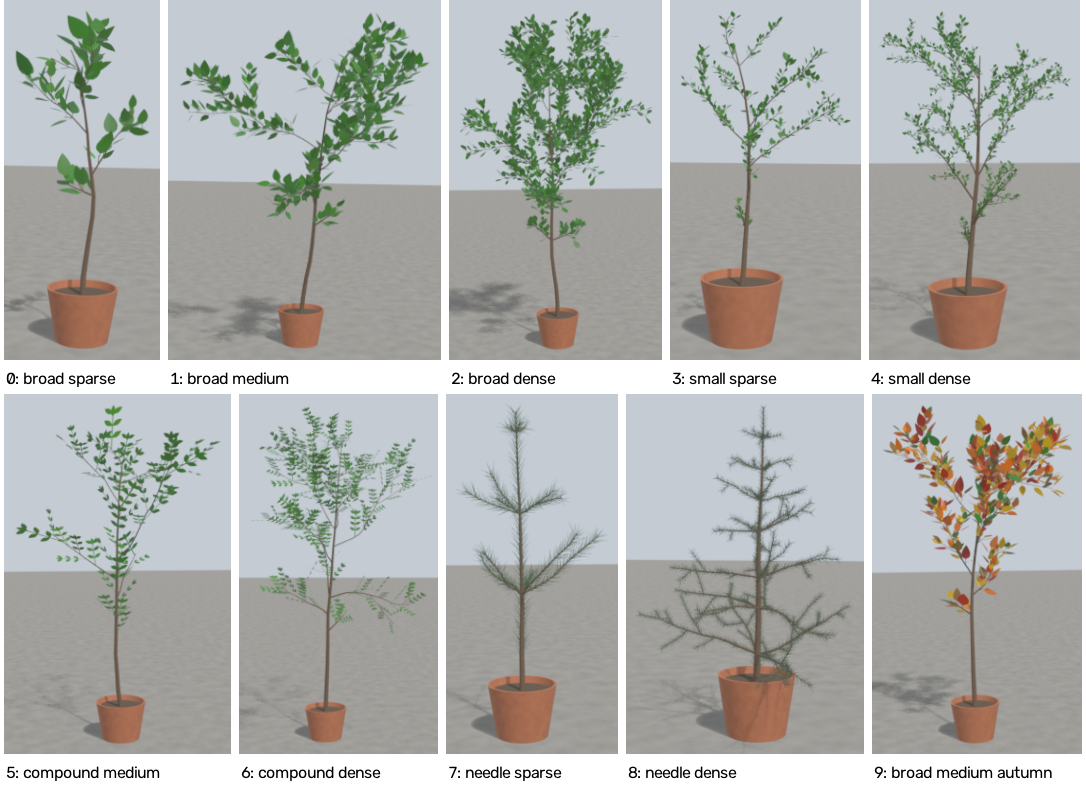
\includegraphics[width=\linewidth]{fig_trees.png}
\caption{The \NTrees{} procedural saplings (calm, first frame): broad, small, pinnate-compound and needle leaves at sparse to dense canopy densities, including an autumn-coloured variant for vegetation-mask robustness. Leaves are real meshes, not alpha-textured cards.}
\label{fig:trees}
\end{figure}

\subsection{Procedural saplings with leaf identities}
Each tree is a skeleton of nodes (position, radius, parent) grouped into branches of increasing order, grown with stochastic wander, phototropic up-turn and phyllotactic or whorled branching \citep{weber1995trees}. Wood is meshed as parallel-transported tubes. Leaf sites are spaced along branch segments; a leaf is attached at the bark surface of a segment and inherits that segment's frame. Leaf blades are real triangulated surfaces with species-dependent outlines (ovate, elliptic, obovate, lanceolate), cupping and droop; compound leaves consist of a rachis and leaflets, and needles are closed triangular prisms. Every leaf has an integer identity, an attachment point, a parent branch, a rest frame, an area and a centroid, stored with the canonical (rest) mesh (\cref{tab:trees}). Heights range from \HeightMin{} to \HeightMax\,m and leaf counts from \NLeavesMin{} to \NLeavesMax{}.

\begin{table}[t]
\centering\small
\caption{Dataset composition. Height includes the pot; triangles count wood and leaves. Trees in the test split are held out for generalisation.}
\label{tab:trees}
\resizebox{\linewidth}{!}{\begin{tabular}{rllrrrrl}
\toprule
ID & Preset & Leaf type & Height (m) & Leaves & Leaf area (m$^2$) & Triangles & Split \\
\midrule
0 & broad\_sparse & broad & 1.00 & 86 & 0.161 & 2{,}890 & train \\
1 & broad\_medium & broad & 1.54 & 624 & 0.874 & 17{,}234 & train \\
2 & broad\_dense & broad & 1.98 & 2{,}591 & 2.460 & 65{,}376 & train \\
3 & small\_sparse & small & 0.87 & 535 & 0.064 & 9{,}190 & train \\
4 & small\_dense & small & 0.82 & 1{,}865 & 0.119 & 29{,}992 & train \\
5 & compound\_medium & compound & 1.44 & 62 & 0.257 & 6{,}378 & train \\
6 & compound\_dense & compound & 1.73 & 217 & 0.505 & 27{,}044 & train \\
7 & needle\_sparse & needle & 1.14 & 1{,}672 & 0.078 & 28{,}107 & train \\
8 & needle\_dense & needle & 1.11 & 8{,}192 & 0.146 & 136{,}748 & test \\
9 & broad\_medium\_autumn & broad & 1.47 & 557 & 0.829 & 15{,}366 & test \\
\bottomrule
\end{tabular}
}
\end{table}

\subsection{Exact procedural wind}
We deliberately do not use physics simulation or a node-based deformer: the same closed-form function both moves the rendered vertices and produces the exported ground truth, so the two are identical by construction.

\paragraph{Branch sway} Every skeleton node $j$ receives a bend rotation
\begin{equation}
\Delta_j(t) = \mathrm{Rot}\big(\mathbf b, \theta_j(t)\big)\,\mathrm{Rot}\big(\mathbf w, \psi_j(t)\big),
\end{equation}
where $\mathbf w$ is the horizontal wind direction and $\mathbf b = \mathbf e_z \times \mathbf w$. Rotations are accumulated from the root by forward kinematics, $A_j = A_{p(j)}\Delta_j$ and $\mathbf p_j = \mathbf p_{p(j)} + A_{p(j)}(\mathbf p_j^0 - \mathbf p_{p(j)}^0)$, so displacement grows with height and branching order. The bend and cross-wind angles are
\begin{align}
\theta_j &= c_j\, g_b(U_e)\,[\alpha_s + \alpha_o \sin(2\pi f_{B}t + \phi_{B})], \\
\psi_j &= c_j\, g_b(U_e)\,\alpha_c \sin(2\pi r f_{B} t + \phi'_{B}),
\end{align}
with frequency $f_B$ and phase $\phi_B$ shared by all nodes of a branch $B$ (coherent sway), and a compliance $c_j \propto (r_0/r_j)\,\ell_j$ that favours thin, long segments.

\paragraph{Leaf flutter} Each leaf rotates rigidly about its petiole attachment,
\begin{equation}
\begin{split}
R_\ell = {}& \mathrm{Rot}(\mathbf m_\ell, g_l\beta_m)\,\mathrm{Rot}\big(\mathbf x_\ell, g_l\beta_t \sin(2\pi r_\ell f_\ell t + \phi'_\ell)\big) \\
& \mathrm{Rot}\big(\mathbf y_\ell, g_l\beta_p\sin(2\pi f_\ell t + \phi_\ell)\big),
\end{split}
\end{equation}
with a per-leaf frequency $f_\ell\in[2.5, 9]$\,Hz, mean down-wind reconfiguration about $\mathbf m_\ell = \mathbf n_\ell \times \mathbf w$, and is carried by its node: $A_\ell = A_{n(\ell)}R_\ell$. The leaf's rigid transform from the canonical pose, $\mathbf x_t = A_\ell \mathbf x_0 + \mathbf t_\ell$, is exported per frame.

\paragraph{Amplitude laws and gusts} $g_b(U) = (U/U_r)^2$ follows the quadratic dependence of drag on speed for small elastic deflections; $g_l(U) = s\tanh\big((U/U_r)/s\big)$ lets flutter grow roughly linearly and saturate. Gusts modulate the speed, $U_e(t) = U\,\max\{0,\,1+\gamma\,n(t)\}$, with a smooth seeded noise $n(t)$. All angles vanish exactly at $U=0$ and rotations are evaluated element-wise, so calm sequences are the rest pose bit-for-bit. Phases depend only on the tree seed, so different wind levels of a tree differ only in amplitude. Over \NFrames{} frames, the median leaf displacement at \WindMax\,m/s ranges from \WindDispHiMin{} to \WindDispHiMax\,mm across trees, with median leaf rotations of \WindRotHiMin--\WindRotHiMax$^\circ$ (\cref{fig:wind}). These amplitudes are configurable and are calibrated against real fan recordings by matching the optical-flow leaf speed per wind level (\cref{sec:calib}). \todo{report calibrated amplitudes.}

\begin{figure}[t]
\centering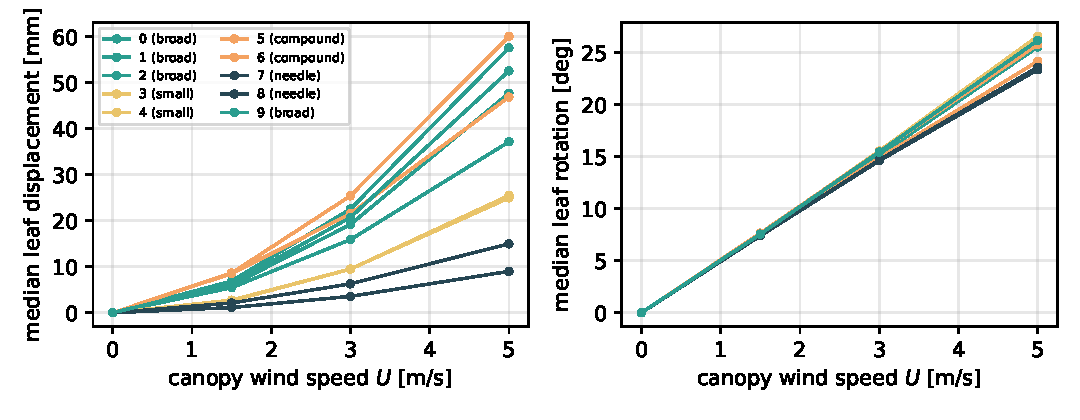
\includegraphics[width=0.9\linewidth]{fig_wind_motion.pdf}
\caption{Ground-truth leaf motion per tree versus canopy wind speed (median over leaves and frames).}
\label{fig:wind}
\end{figure}

\subsection{Sensor-matched rendering and ground-truth passes}
The camera reproduces the real sensor's pinhole intrinsics exactly (focal length, principal point via lens shift, pixel aspect) and a hand-held orbit with seeded smooth jitter; the trajectory depends only on the tree seed, so it is bit-identical across wind levels. Time is explicit: frame $i$ is rendered at $t = i\,k/\text{fps}$ for both wind and camera.

RGB is rendered with EEVEE or Cycles and converted to 8-bit sRGB with the exact transfer function. Ground truth is rendered in a separate Cycles pass with one sample per pixel and a 0.01-pixel box filter, so every value is the first hit of the ray through the pixel centre and is never blended across edges. Shader outputs store per-pixel world position, normal, leaf identity, semantic class, rest position and next-frame position. Depth is computed as $z = (\mathbf P - \mathbf C)\cdot \mathbf o$ from the world position, so it is z-depth by construction. Exact optical flow is obtained by projecting the interpolated next-frame position, which also covers non-rigid wood deformation. Motion blur and rolling shutter are optional and are rendered by sub-frame and row-band integration.

\begin{figure}[t]
\centering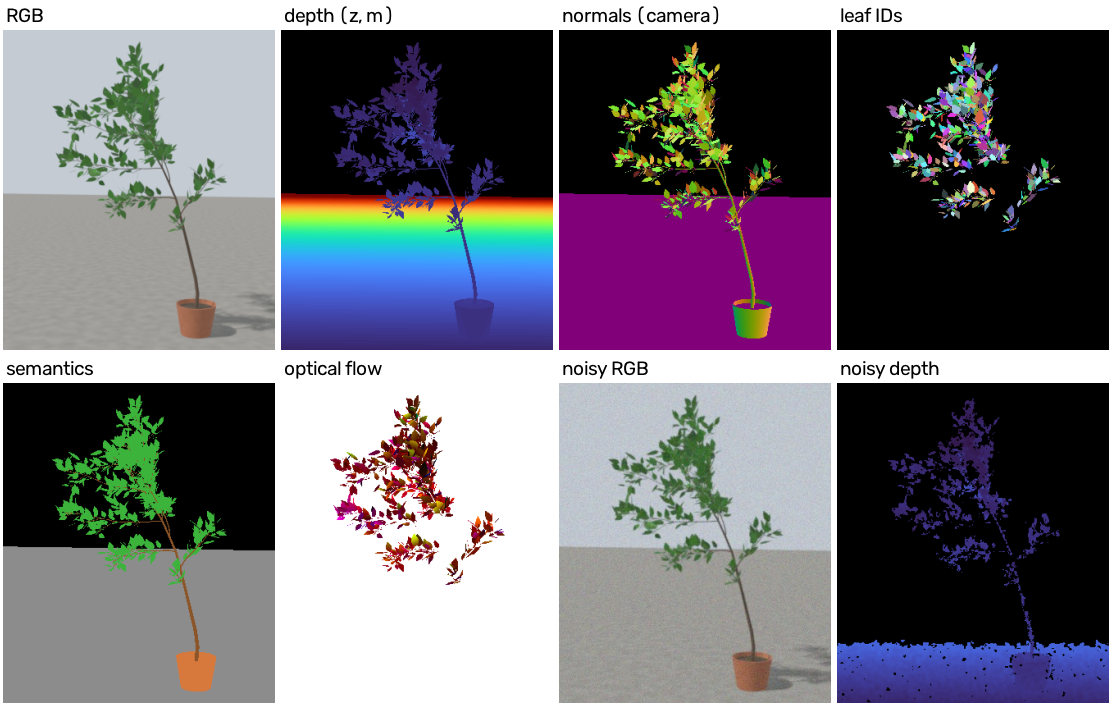
\includegraphics[width=\linewidth]{fig_modalities.png}
\caption{Per-frame products for a broad-leaved sapling at $U=\WindMax$\,m/s. Clean products are exact; noisy RGB and depth follow the sensor model of \cref{sec:noise}.}
\label{fig:modalities}
\end{figure}

\subsection{Sensor noise model}\label{sec:noise}
Clean data are always kept and a noisy copy is derived. Depth undergoes resampling to the sensor's effective depth resolution; spatially correlated noise with $\sigma(z) = a + b z^2$ or, alternatively, Gaussian disparity noise with sub-pixel quantisation; flying pixels that interpolate foreground and background depth at discontinuities; holes whose probability increases near edges, on structures thinner than a few pixels and at grazing angles; range limits; misregistration; and quantisation to millimetres. RGB receives an auto-exposure random walk, slight blur, shot and read noise and JPEG compression. Noise draws are keyed to the tree and frame, so they are paired across wind levels.

\subsection{Calibration against the real sensor}\label{sec:calib}
The noise parameters are fitted from real recordings of a flat textured wall at six distances (plane-fit residuals give $a$, $b$ and the spatial correlation; invalid pixels give the random hole rate) and of real leaves against a distant background (vegetation silhouettes give flying-pixel, edge-hole and thin-structure-hole rates by fixed-point matching of simulated statistics). On synthetic recordings with known parameters, the procedure recovers $a$, $b$ and the correlation length within 3\,\% and the flying-pixel and hole rates within 2\,\%. Wind amplitudes are calibrated analogously by matching the median metric leaf speed (optical flow scaled by depth) of real static-camera fan clips, iterating until all wind levels agree within 3\,\%; a self-test with a known amplitude factor of 1.6 recovers 1.57. \todo{insert real-sensor calibration results and plots.}

\subsection{Validation}
Every sequence is validated automatically on the exported products (\cref{tab:validation}); all \NSeqPassed{} of \NSeqValidated{} sequences pass. The decisive check for depth convention is geometric: back-projecting the depth of the floor yields points within \ValGroundUm\,$\mu$m of the plane $z=0$ even in the image corners, whereas interpreting the same values as ray distance would displace them by \ValRayMm\,mm.

\begin{table}[t]
\centering\small
\caption{Automatic validation over all released sequences.}
\label{tab:validation}
\resizebox{\linewidth}{!}{\begin{tabular}{llr}
\toprule
Check (all 40 sequences) & Statistic & Value \\
\midrule
World position re-projects onto its own pixel centre & max error & 0.0036 px \\
Cross-frame re-projection of exported depth (static geometry) & worst median & 0.002 px \\
Back-projected floor lies on $z=0$ (image corners) & worst median & 3 $\mu$m \\
\quad same test if depth were ray distance & median & 147 mm \\
16-bit PNG depth vs.\ float EXR depth & max difference & 0.50 mm \\
Leaf-ID pixels not in table / inconsistent with semantics & total & 0 px \\
Per-leaf transforms predict rendered flow (leaf pixels) & worst median & 0.007 px \\
Rendered flow of static geometry & worst median & 0.006 px \\
\bottomrule
\end{tabular}
}
\end{table}

% ======================================================================
\section{Benchmark protocol}\label{sec:protocol}
\paragraph{Data and splits} Each tree is rendered calm and at \WindLevels\,m/s along a single orbit of \NFrames{} frames at the real sensor's resolution. Every eighth frame is held out for view-synthesis evaluation, and two trees are held out entirely for generalisation studies.

\paragraph{Methods} We evaluate splatfacto (3DGS) and depth-nerfacto (NeRF with depth supervision) from Nerfstudio \citep{tancik2023nerfstudio}, trained with the ground-truth poses in metric world coordinates (no re-centring or re-scaling) and initialised from back-projected sensor depth of the same variant (clean or noisy). \todo{add a dynamic method (e.g. 4D Gaussians) and a simple mitigation.}

\paragraph{Geometry-first evaluation} Reconstructions are compared with the canonical leaf surface. Each reconstructed point is attributed to its nearest ground-truth surface (leaf, wood, pot/soil or floor); points farther than 3\,cm from every surface are floaters and are reported separately. For Gaussians, precision-side quantities (accuracy, precision, floaters, per-leaf centroids, leaf angles) use Gaussian centres, so each splat counts once, whereas coverage-side quantities (completeness, recall, recovered leaf area, leaf coverage) use samples spread over each Gaussian's footprint, because centres alone under-cover thin surfaces. We report the F-score at $\tau = 5$\,mm, a capped chamfer distance, the relative leaf-area error, the 1-D Wasserstein distance between leaf inclination distributions \citep{ross1981radiation}, and the median per-leaf centroid error. Needles are thinner than a pixel, so for conifers per-leaf quantities are computed per shoot (all needles of a twig). View-synthesis PSNR is reported on held-out views.

\paragraph{Three-way decomposition} For a metric $E$ oriented so that larger is worse,
\begin{align}
E_{\text{method}} &= E(\text{calm}, \text{clean}), \\
E_{\text{sensor}} &= E(\text{calm}, \text{noisy}) - E(\text{calm}, \text{clean}), \\
E_{\text{wind}}(U) &= E(U, \text{noisy}) - E(\text{calm}, \text{noisy}), \\
E_{\text{int}}(U) &= \big[E(U,\text{noisy}) - E(U,\text{clean})\big] - E_{\text{sensor}}.
\end{align}
The interaction term measures how far sensor and wind errors are from additive. Values are averaged over seeds per configuration, and mean and standard deviation over trees are reported.

% ======================================================================
\section{Results}\label{sec:results}
\todo{Provisional: \NResultRuns{} runs on \NResultTrees{} trees with \NResultSeeds{} seed(s); final tables are regenerated automatically from the full multi-seed, multi-method benchmark.}

\begin{table}[t]
\centering\small
\caption{Benchmark results, mean over trees (and seeds). CD: capped chamfer distance; Area err: relative leaf-area error; Angle W1: leaf inclination distribution distance.}
\label{tab:results}
\resizebox{\linewidth}{!}{\begin{tabular}{llrrrrrrr}
\toprule
Method & Condition & F@5mm$\uparrow$ & CD [mm]$\downarrow$ & Centroid [mm]$\downarrow$ & Area err$\downarrow$ & Angle W1 [deg]$\downarrow$ & Floaters$\downarrow$ & PSNR [dB]$\uparrow$ \\
\midrule
splatfacto & calm / clean & 0.392 & 19.0 & 2.8 & 0.59 & 13.8 & 0.18 & 39.3 \\
 & calm / noisy & 0.441 & 17.9 & 3.8 & 0.43 & 13.4 & 0.31 & 29.4 \\
 & low / noisy & 0.306 & 19.7 & 7.1 & 0.56 & 15.4 & 0.34 & 28.8 \\
 & medium / noisy & 0.200 & 21.2 & 8.1 & 0.69 & 17.6 & 0.34 & 28.1 \\
 & high / noisy & 0.133 & 24.4 & 13.7 & 0.79 & 18.4 & 0.40 & 27.5 \\
 & high / clean & 0.124 & 24.7 & 14.1 & 0.83 & 16.7 & 0.21 & 30.3 \\
\bottomrule
\end{tabular}
}
\end{table}

\paragraph{Calm and clean (occlusion/method error)} Even with exact poses and noise-free depth, splatfacto reaches only F@5mm = \SpBaseF{} and a chamfer distance of \SpBaseCD\,mm on leaves (\cref{tab:decomp}), and inclines leaves more steeply than they are; this is the intrinsic difficulty of thin, self-occluding foliage.

\paragraph{Wind} Wind is the dominant degradation. At \WindMax\,m/s the leaf F-score drops by \SpWindHiF{}, the chamfer distance increases by \SpWindHiCD\,mm and the per-leaf centroid error by \SpWindHiCentroid\,mm, monotonically with wind speed (\cref{fig:decomp}).

\paragraph{Sensor} With the current (uncalibrated) sensor model, the sensor term is small (\SpSensorF{} in F-score, \SpSensorCD\,mm in chamfer distance) and of the order of the training variability between seeds (\SpSeedStdF{} in F-score). \todo{re-evaluate with the calibrated noise profile; a negative sensor term must be confirmed or explained.}

\paragraph{Interaction} The interaction at \WindMax\,m/s is \SpInterHiCD\,mm in chamfer distance, small relative to the wind term, so the decomposition is approximately additive in this regime.

\begin{table}[t]
\centering\small
\caption{Three-way error decomposition (mean $\pm$ std over trees). $^{\dagger}$Absolute baseline values; other rows are increases in error (decrease for F-score).}
\label{tab:decomp}
\begin{tabular}{llrrr}
\toprule
Method & Component & $\Delta$F@5mm & $\Delta$CD [mm] & $\Delta$Centroid [mm] \\
\midrule
depth-nerfacto & Occlusion/method$^{\dagger}$ & 0.558 $\pm$ 0.078 & 6.4 $\pm$ 0.6 & 5.6 $\pm$ 1.5 \\
 & Sensor & +0.033 $\pm$ 0.090 & +0.2 $\pm$ 1.1 & +1.0 $\pm$ 0.3 \\
 & Wind, $U=1.5$ m/s & +0.101 $\pm$ 0.045 & +1.0 $\pm$ 0.4 & +1.8 $\pm$ 0.2 \\
 & Wind, $U=3$ m/s & +0.374 $\pm$ 0.009 & +13.1 $\pm$ 7.1 & +7.6 $\pm$ 3.1 \\
 & Wind, $U=5$ m/s & +0.348 $\pm$ 0.063 & +10.3 $\pm$ 0.7 & +11.6 $\pm$ 3.9 \\
 & Interaction, $U=5$ & -0.018 $\pm$ 0.089 & +2.2 $\pm$ 3.1 & +2.6 $\pm$ 4.5 \\
\midrule
splatfacto & Occlusion/method$^{\dagger}$ & 0.379 $\pm$ 0.117 & 19.3 $\pm$ 4.1 & 6.7 $\pm$ 5.7 \\
 & Sensor & -0.060 $\pm$ 0.055 & -1.5 $\pm$ 1.5 & +1.9 $\pm$ 3.1 \\
 & Wind, $U=1.5$ m/s & +0.134 $\pm$ 0.073 & +1.5 $\pm$ 0.4 & +2.2 $\pm$ 1.8 \\
 & Wind, $U=3$ m/s & +0.272 $\pm$ 0.112 & +4.3 $\pm$ 1.8 & +5.2 $\pm$ 6.7 \\
 & Wind, $U=5$ m/s & +0.341 $\pm$ 0.131 & +8.1 $\pm$ 4.7 & +12.0 $\pm$ 8.5 \\
 & Interaction, $U=5$ & +0.059 $\pm$ 0.054 & +1.4 $\pm$ 1.5 & -0.8 $\pm$ 2.1 \\
\bottomrule
\end{tabular}

\end{table}

\begin{figure}[t]
\centering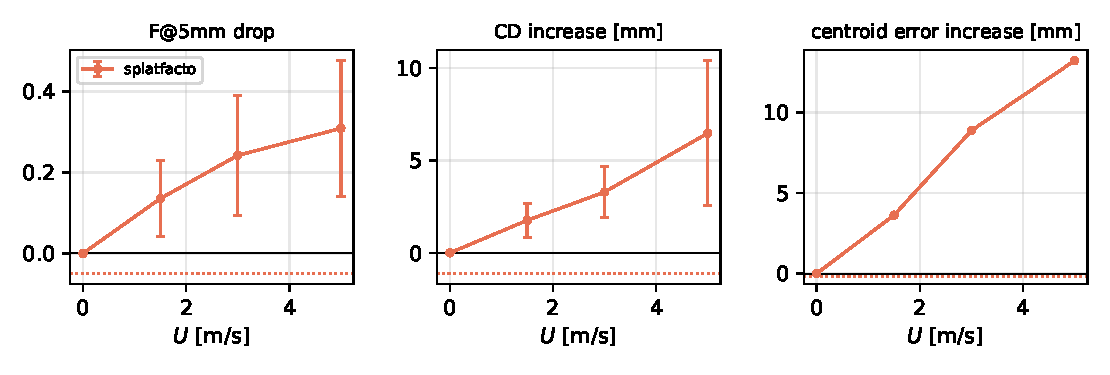
\includegraphics[width=\linewidth]{fig_decomposition.pdf}
\caption{Wind error versus canopy wind speed (mean $\pm$ std over trees); dotted lines mark the sensor error.}
\label{fig:decomp}
\end{figure}

\paragraph{View synthesis hides geometric damage} From calm to \WindMax\,m/s, PSNR on held-out views changes by \RelChangePSNR\,\% while the leaf F-score changes by \RelChangeF\,\% (\cref{fig:imggeo}). Methods that average moving leaves into blurred but plausible appearance are rewarded by image metrics; per-leaf geometric ground truth is needed to expose the error.

\begin{figure}[t]
\centering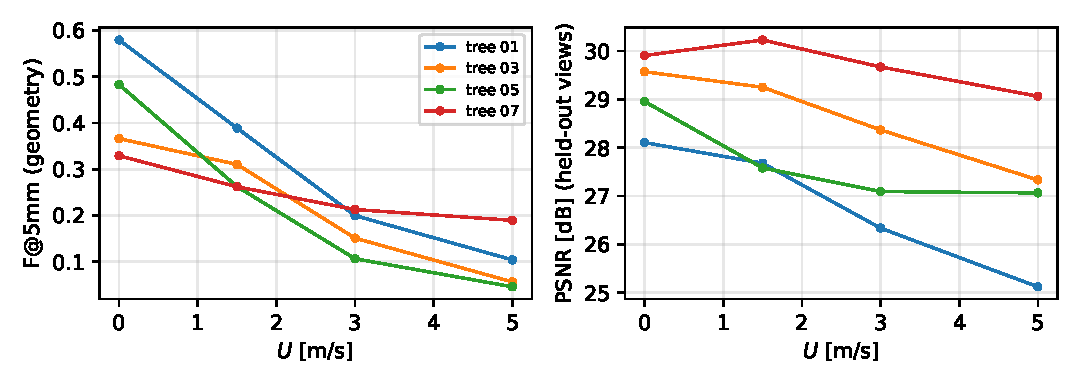
\includegraphics[width=0.9\linewidth]{fig_image_vs_geometry.pdf}
\caption{Geometry (left) versus view-synthesis quality (right) under increasing wind, splatfacto, noisy sensor.}
\label{fig:imggeo}
\end{figure}

\paragraph{Real data} \todo{reconstruction of the real saplings at the same wind levels; real-vs-synthetic agreement of the error-versus-$U$ trend.}

% ======================================================================
\section{Discussion and limitations}
The generator trades biomechanical fidelity for exactness: branch bending is piecewise rigid along skeleton segments, compound leaves move as single rigid units, leaves may interpenetrate, gusts are spatially uniform, and wind amplitudes and noise parameters must be calibrated to the target setup (\cref{sec:calib}). Motion blur and rolling shutter affect RGB only; ground truth refers to the frame-centre time, as for a global-shutter depth sensor. Rendered pixels are deterministic per machine but not across GPUs, whereas geometry, poses and ground truth are bit-identical. The benchmark currently covers static-scene methods; dynamic reconstructions are the natural next step, and the exported per-leaf transforms and optical flow allow their motion to be evaluated directly.

\section{Conclusion}
SynthTree provides paired calm/windy RGB-D sequences of plants with exact per-leaf ground truth and a protocol that separates occlusion, sensor and wind error. First results indicate that wind, not sensor noise, is the dominant source of geometric error for neural foliage reconstruction, and that image-space metrics conceal most of it.

\section*{Data and code availability}\label{sec:availability}
Code: \url{https://github.com/bibekgyawali2/synthtree}. Dataset: \todo{public Kaggle/Zenodo DOI} (CC BY 4.0).

\section*{CRediT authorship contribution statement}
\todo{}

\section*{Declaration of competing interest}
The authors declare no competing interests.

\bibliographystyle{elsarticle-harv}
\bibliography{refs}
\end{document}
